\documentclass[a4paper]{article}

%% Language and font encodings
\usepackage[french]{babel}
\usepackage[utf8x]{inputenc}
\usepackage[T1]{fontenc}

%% Sets page size and margins
\usepackage[a4paper,top=3cm,bottom=3cm,left=2cm,right=2cm,marginparwidth=2cm]{geometry}

%% Useful packages
\usepackage{amsmath}
\usepackage{graphicx}
\usepackage[colorinlistoftodos]{todonotes}
\usepackage[colorlinks=true, allcolors=black]{hyperref}
\usepackage{fourier-orns}
\usepackage{titlesec}
\usepackage{fancyhdr}
\usepackage{fancyvrb}
\usepackage{float}
\pagestyle{fancy} 
\setcounter{tocdepth}{5}

%% Tikz stuff
\usepackage{tikz}
\usetikzlibrary{calc, arrows}
\tikzstyle{incolore} = [rectangle, rounded corners, draw=black, minimum height=1cm, minimum width=3cm, text width=3cm, text centered]

\usepackage{libertine}
\newcommand{\hsp}{\hspace{20pt}}
\newcommand{\HRule}{\rule{\linewidth}{0.5mm}}

\renewcommand{\headrulewidth}{1pt}
\fancyhead[C]{}
\fancyhead[L]{}
\fancyhead[R]{\footnotesize{\leftmark}}

\renewcommand{\footrulewidth}{1pt}
\fancyfoot[C]{}
\fancyhead[L]{}
\fancyfoot[R]{\thepage}

\definecolor{Zgris}{rgb}{0.87,0.85,0.85}

\usepackage{eso-pic,graphicx}
\usepackage{xcolor}
\newcommand{\bgimg}[1]
{
    \AddToShipoutPicture
    {
        \put(\LenToUnit{0 cm},\LenToUnit{0 cm})
        {
            \includegraphics[width=\paperwidth,height=\paperheight]{#1}
        }
    }
}

\usepackage{xcolor}
\usepackage{listings}

\definecolor{mGreen}{rgb}{0,0.6,0}

\lstdefinestyle{CStyle}{
    commentstyle=\color{mGreen},
    keywordstyle=\color{red},
    numberstyle=\color{gray},
    stringstyle=\color{purple},
    frame=single,
    breakatwhitespace=false,
    breaklines=true,
    captionpos=b,
    keepspaces=true,
    numbers=left,
    showspaces=false,
    showstringspaces=false,
    showtabs=false,
    tabsize=2,
    language=C
}

\begin{document}





\begin{titlepage}
    \begin{sffamily}
        \begin{center}

            
\includegraphics[width=5cm]{images/LogoHenallux.PNG}~\\[1.5cm]
            \textsc{\Large Rapport de projet}\\[1.5cm]

            \HRule \\[0.4cm]
            { \huge \bfseries Implémentation d'un IDS \\[0.4cm] }
            \HRule \\[2cm]

            \begin{minipage}{0.4\textwidth}
                \begin{flushleft} \large
                    Grégoire Roumache\\
                    Florian Fichet\\
                \end{flushleft}
            \end{minipage}
            \begin{minipage}{0.55\textwidth}
                \begin{flushright} \large
                    Développement -- Sécurité des systèmes\\
                    Deuxième année, groupe C-2 \\
                    Année académique 2020-2021\\
                \end{flushright}
            \end{minipage}
            \vfill

            {\large 3 Janvier 2021}

        \end{center}
    \end{sffamily}
\end{titlepage}

\let\cleardoublepage\clearpage










\section{Introduction}





Pour le cours de Développement, nous avons dû implémenter un IDS (Intrusion Detection System) qui analyse le trafic qui passe par une interface réseau de la machine. Il permet de détecter des activités suspectes en fonction d'un certain nombre de règles données au préalable. En cas d'anomalie, le programme peut alerter l'utilisateur en la signalant dans les logs du système.

Nous nous sommes organisés en utilisant la plateforme github, comme recommandé, et voici le lien vers notre répertoire: 
\begin{center}
    {\small \url{https://github.com/groumache/Intrusion-Detection-System}}
\end{center}










\section{Organisation du travail et configuration des outils}





\subsection{Les issues sur github}



Les issues sont utilisées pour s'organiser et garder une trace des tâches, des améliorations et des bugs dans un projet sur github.
\begin{figure}[H]
    \centering
    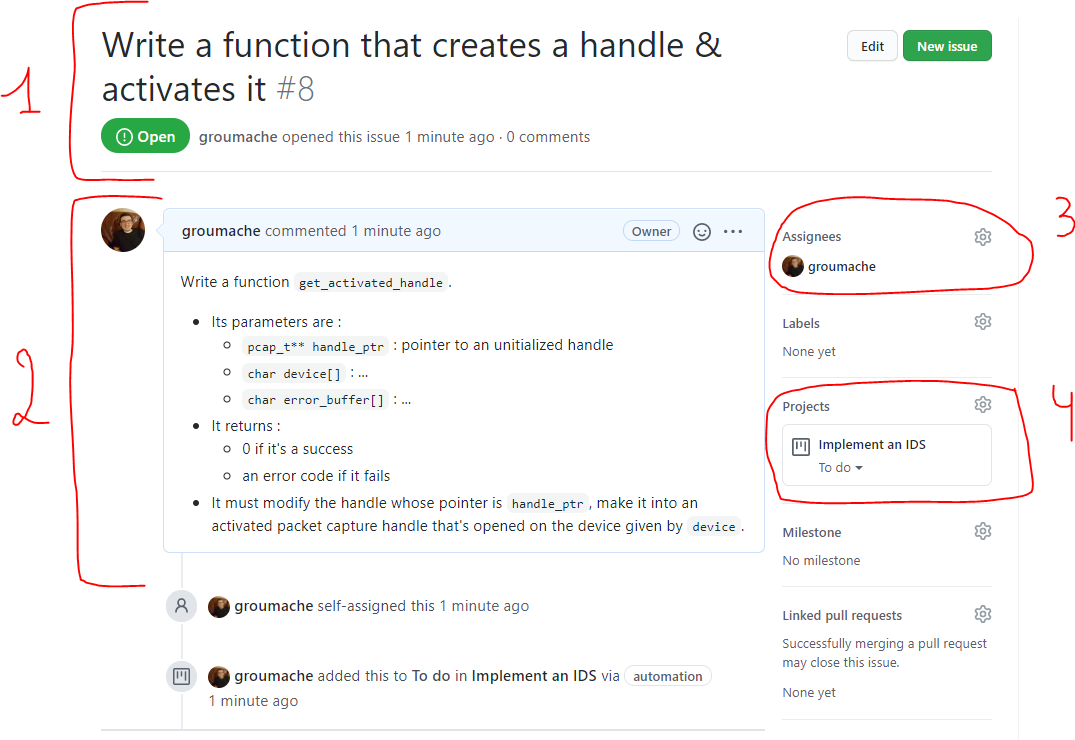
\includegraphics[width=0.99\linewidth]{../markdown-explanations/images/issue-1.PNG}
    \caption{Une issue sur github}
    \label{fig:issue01}
\end{figure}
Explication de la figure \ref{fig:issue01}:
\begin{enumerate}
    \item Titre de l'issue.
    \item Explication/description de l'issue.
    \item On peut attribuer une issue à des personnes qui seront responsables pour résoudre l'issue.
    \item Le projet dans lequel l'issue va apparaître.
\end{enumerate}





\subsection{Utilisation du kanban sur github}



Comme nous l'avons précisé dans l'introduction, nous nous sommes organisés en utilisant github. Nous n'avons pas seulement mis le code sur github mais aussi utilisé le tableau kanban avec 4 sections:
\begin{enumerate}
    \item \textbf{Ideas}: un endroit pour ajouter des notes/issues qui dépassent les exigences du projet.
    \item \textbf{To do}: un endroit où les issues sont placées quand elles sont créées (correspond aux critères minimum de réussite).
    \item \textbf{In progress}: l'endroit où les issues vont quand on travaille dessus.
    \item \textbf{Done}: là où les issues vont quand elles sont fermées ou la pull request liée a été fusionnée.
\end{enumerate}
\begin{figure}[H]
    \centering
    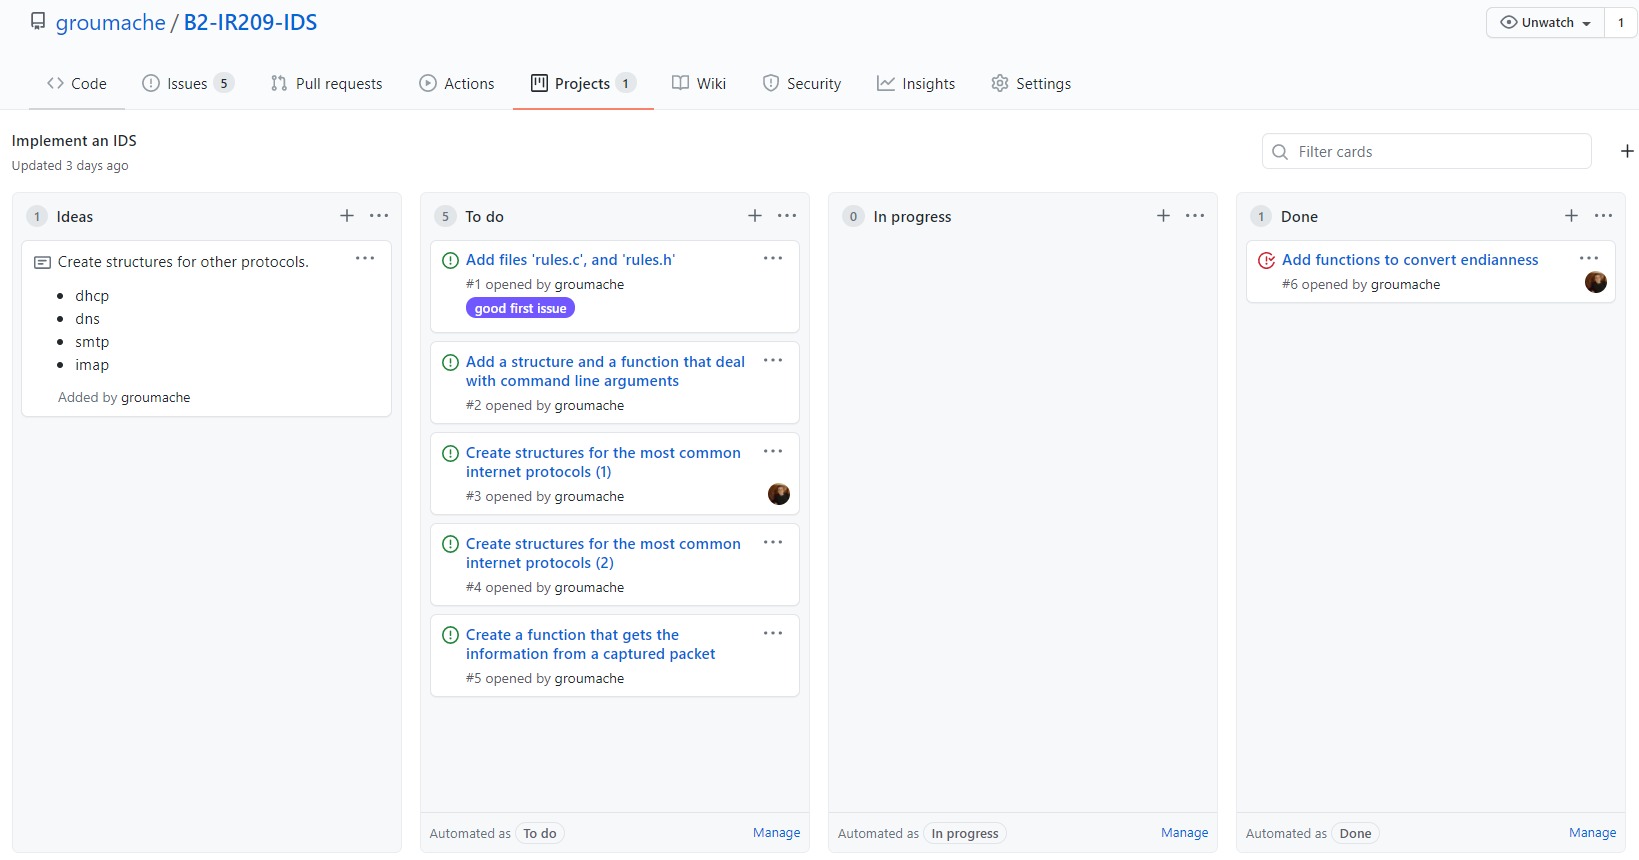
\includegraphics[width=0.99\linewidth]{../markdown-explanations/images/project-1.PNG}
    \caption{Kanban sur github}
\end{figure}

Sur le schéma de la figure \ref{fig:networkgraph}, on voit le network graph. Cette image illustre bien comment nous avons travaillé, c-à-d en créant des nouvelles branches à chaque fois que nous avons eu besoin de résoudre une issue. Une fois que le code a été ajouté, nous avons fait des pull requests pour fusionner les branches.
\begin{figure}[H]
    \centering
    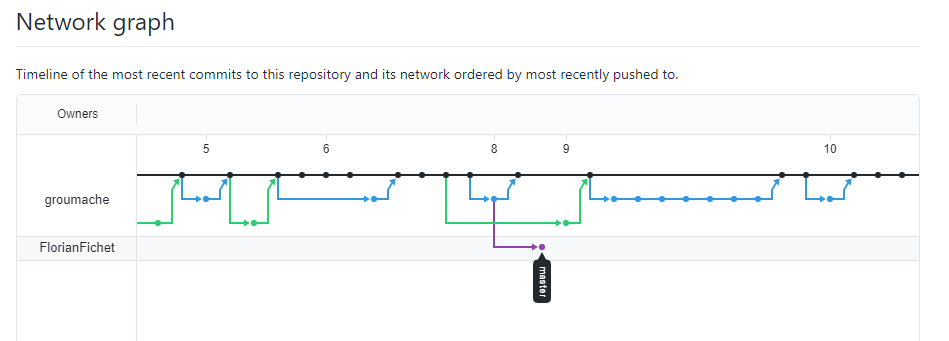
\includegraphics[width=0.99\linewidth]{../markdown-explanations/images/project-2.PNG}
    \caption{Network graph montrant les commits et comment les branches se rejoignent}
    \label{fig:networkgraph}
\end{figure}





\subsection{Configuration du debugger et utilisation de valgrind}



Les fichiers de configurations sont présentés sur les figures \ref{fig:debugconfig1} et \ref{fig:debugconfig2}.
\begin{enumerate}
    \item Sur la figure \ref{fig:debugconfig1}, on voit le fichier \textit{tasks.json} où on configure la compilation du projet:
    \begin{itemize}
        \item on voit que le paramètre \textit{command} donne bien le compilateur gcc,
        \item les arguments sont précisés par le paramètre \textit{args}, ce sont ceux recommandés dans l'énoncé,
        \item si on combine le tout, c'est l'équivalent de la commande:
        \begin{center}
            \texttt{\small gcc -Wall -o ids main.c populate.c rules.c -lpcap}
        \end{center}
    \end{itemize}
    \item Sur la figure \ref{fig:debugconfig2}, on voit le fichier \textit{launch.json}, il sert à configurer le lancement du programme:
    \begin{itemize}
        \item dans \textit{program}, on voit qu'on a bien précisé \textit{ids},
        \item et dans \textit{args}, on voit les arguments du programme.
        \item si on combine le tout, c'est l'équivalent de la commande:
        \begin{center}
            \texttt{\small ids -p -d eth1 -r ids.rules -n 10}
        \end{center}
    \end{itemize}
\end{enumerate}
Remarquez qu'il faut lancer le programme avec des privilèges plus élevé que l'utilisateur standard. Pour réussir à faire cela, on peut lancer visual studio code avec ces mêmes privilèges.
\begin{figure}[H]
    \centering
    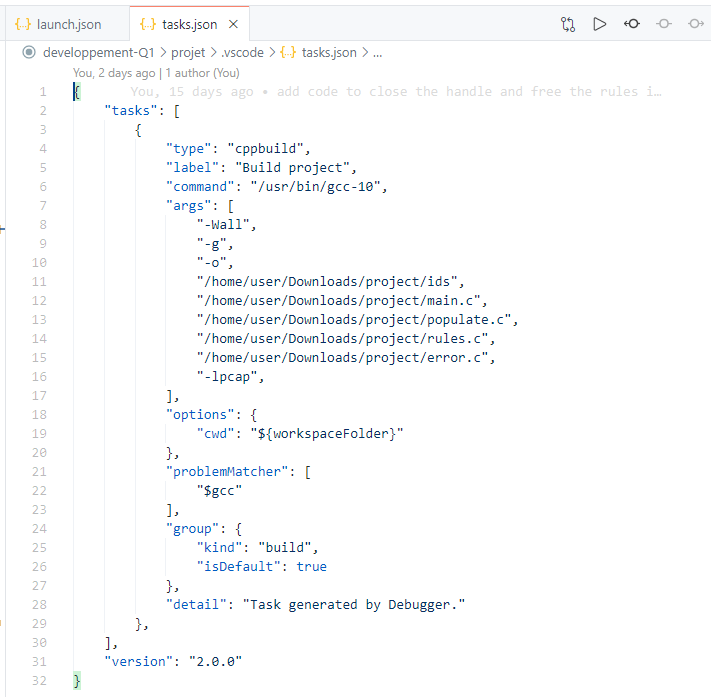
\includegraphics[width=0.65\linewidth]{images/task-json.PNG}
    \caption{Fichier de configuration du debugger, pour la compilation du programme}
    \label{fig:debugconfig1}
\end{figure}
\begin{figure}[H]
    \centering
    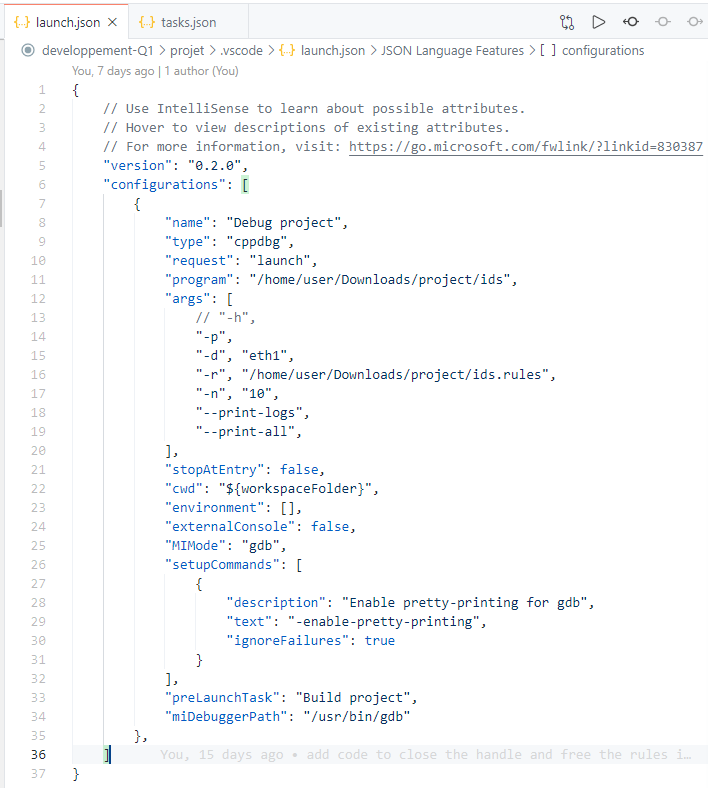
\includegraphics[width=0.70\linewidth]{images/launch-json.PNG}
    \caption{Fichiers de configuration du debugger, pour lancer le programme}
    \label{fig:debugconfig2}
\end{figure}





\subsection{Configuration du formatage automatique}



L'extension C/C++ de visual studio code nous permet de faire du formatage automatique de notre code comme illustré par la figure \ref{fig:formatting}. La configuration se fait au en suivant la syntaxe clang-format, voici celle que nous avons utilisé:

{\small\begin{verbatim}
{
    BasedOnStyle: Google,
    IndentWidth: 4,
    MaxEmptyLinesToKeep: 2,
    IndentPPDirectives: BeforeHash
}
\end{verbatim}}

\begin{figure}[H]
    \centering
    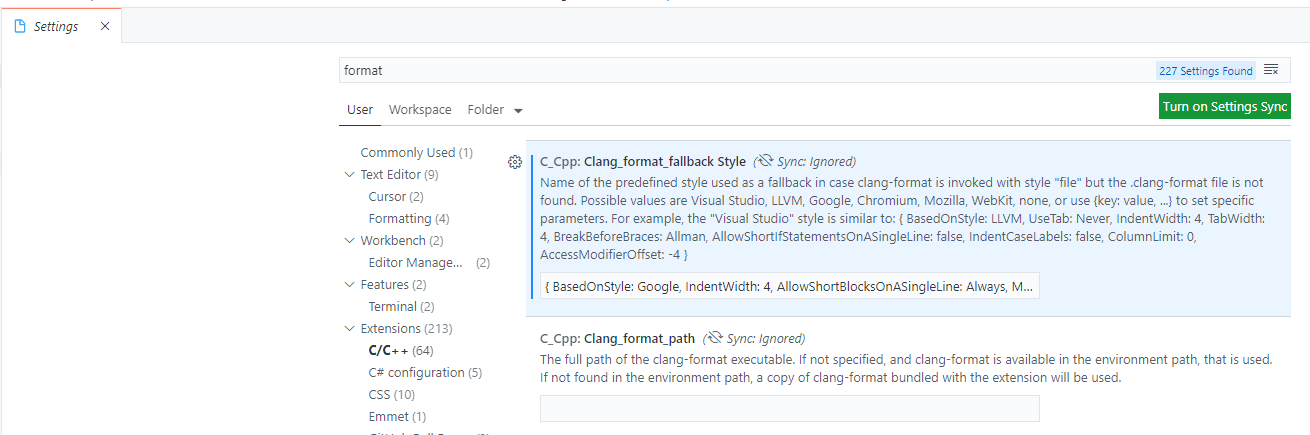
\includegraphics[width=0.99\linewidth]{../markdown-explanations/images/setup-04.PNG}
    \caption{Paramètre de formatage dans visual studio code}
    \label{fig:formatting}
\end{figure}










\section{Architecture du système}





%%










\section{Explication générale sur le fonctionnement du code}





%% /!\ /!\ /!\ EXPLIQUER QUE LES CHOIX D'IMPLÉMENTATION SONT DANS LA SECTION SUIVANTE










\section{Choix d'implémentation spécifiques et problèmes rencontrés}





%%
%% - expliquer le problème avec les structures
%% - expliquer les fonctions récursives
%% - expliquer les fonctions qui changent l'endianness
%% - expliquer les macros avec les masques
%% - expliquer les endroits où j'ai utiliser un shift de bits (<<)
%%

Voici hello world:

\begin{lstlisting}[style=CStyle]
#include <stdio.h>

// this is hello world
int main(void)
{
    printf("Hello World!"); 
}
\end{lstlisting}










\section{Conclusion}





%%















\newpage \tableofcontents \listoffigures
\begin{thebibliography}{9}
\bibitem{1} {\small \url{https://github.com/groumache/Intrusion-Detection-System}}
% \bibitem{2} 
% \bibitem{3} 
% \bibitem{4} 
% \bibitem{5} 
% \bibitem{6} 
\end{thebibliography}




















\end{document}
